% - - - - - - - - - - - - - - - - - - - - - - - - - - - - 
\subsection{PROC-02 Contratar a nuevo personal}

\begin{figure}[htbp]
	\begin{center}
		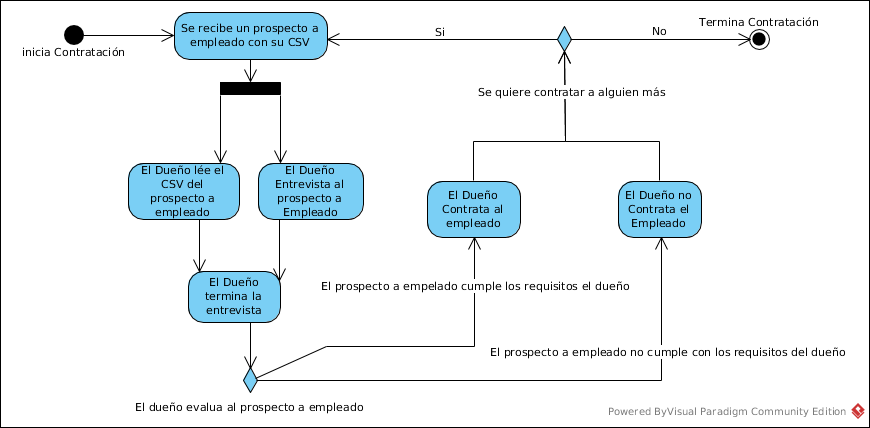
\includegraphics[width=.8\textwidth]{images/AS-toprocContratacion}
		\caption{PROC-02 Contratar a nuevo personal}
		\label{fig:proceso2}
	\end{center}
\end{figure}

\begin{description}
	\item[Descripción:] Cuando se abre una sucursal o simplemente hace falta personal, se procede a contratar a nuevo ya sea supervisor o solo empleado de planta. El Dueño es el que se encarga de la entrevista y de todo el proceso de la contratación.
	\item[Entradas:] \cdtEmpty
        \begin{itemize}
			\item Datos del prospecto a empleado
			\item Un nuevo empleado
        \end{itemize}
	\item[Salidas:] \cdtEmpty
        \begin{itemize}
			\item Contrato
        \end{itemize}	
    \item[Áreas de oportunidad:] Con el sistema funcionando, se facilitará la asignación de una sucursal a un empleado así como guardar los datos del empleado, y también ayudara al dueño a conocer y controlar de mejor forma a su personal.
\end{description}

